By following the architecture proposed in section \ref{sec:system_architecture} and illustrated in figure \ref{fig:sa_design}, the developed system consists of two web applications: the CSA and SSA. The CSA is the application responsible for rendering the User Interface, allowing the definition of user requests, which are processed by the SSA. Thus, although these two applications run separately, the CSA is dependent upon the SSA. 

%The developed applications are divided into two distinct groups: the Client Side Application (CSA), or the User Interface, and the Server Side Application , or the flight data/optimization API. Both applications run independently from one another, although the CSA is dependent of the API, and must communicate with it as to obtain solutions to the user requests. Figure \ref{fig:system_architecture} introduces the architecture of the system, as well as the technologies on which the system relies, which will be addressed in the rest of this section. 


The developed applications, denoted Bfly App and Bfly API, are hosted on \textit{Heroku}, a cloud platform which, upon request, creates two separate runtime environments, one for each application. Each application requires a server to listen to requests and serve content. In particular, the CSA and SSA run on \textit{node.js} and \textit{django} servers, respectively (see figure \ref{fig:sa_structure}. Furthermore, since the User Interface will render a map, the CSA requires access to the Google Maps API. To enable the implementation of a modern web application, the CSA also uses several other frameworks, in particular, React and Redux. In its turn, the SSA requires access to real flight data and thus, will interact with Kiwi's flight data API. The described application structured is illustrated in figure \ref{fig:sa_structure}, and the developed applications are denoted by \textit{Bfly App} and \textit{Bfly API}, for the CSA and SSA, respectively. The previously mentioned underlying technologies will be discussed with further detail in the following subsection.  


%\todo{Edit image. Try to reduce size. Change "cloud platform" to "host". Replace bootstrap to Google modular design}

\begin{figure}[htpb]
  \centering
  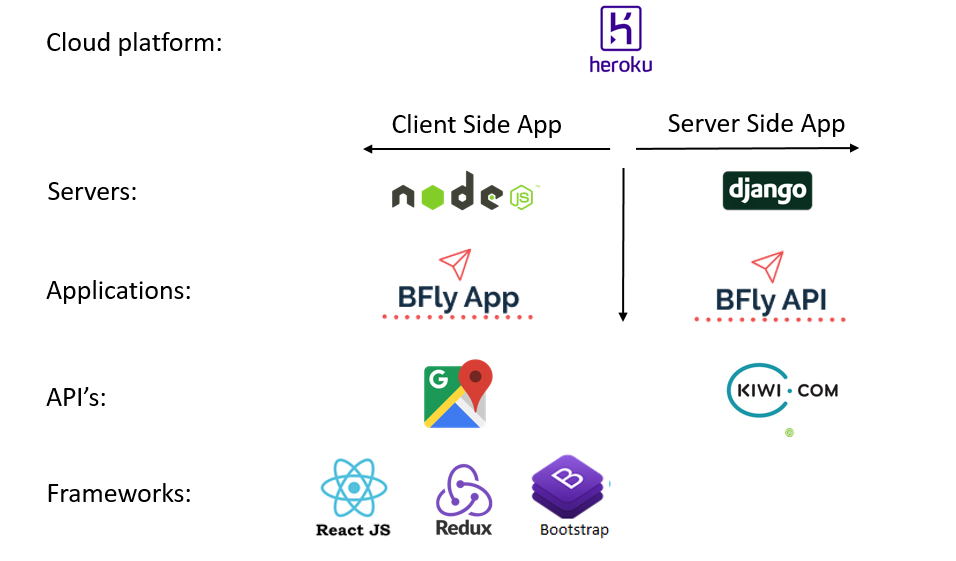
\includegraphics[width=.7\textwidth]{./Figures/system_implementation/system_architecture_implementation.png}
  \caption{Technology stack used by the developed application.}
  \label{fig:sa_structure}  
\end{figure}


%The developed applications run on \textit{Heroku}, a Cloud Platform as a service, which, upon request, creates two separate servers, one for each application. The Client Side Application runs a \textit{Node.Js} server, which creates a bundle file, that is served to the user, and contains all the necessary information to render the UI, handle the user input logic, and interact with the API. In its turn, the API runs on \textit{Django}, which interacts with the webserver to read the user request, and may execute particular instructions according to the selected route.